\documentclass{beamer}

\usepackage{fontspec}
\usepackage{xeCJK}
\setCJKmainfont[BoldFont=Noto Serif CJK TC Bold]{Noto Serif CJK TC}
\XeTeXlinebreaklocale "zh"
\XeTeXlinebreakskip = 0pt plus 1pt
\linespread{1.3}
\allowdisplaybreaks

\usepackage{color}
\usepackage{booktabs}
\usepackage{tabularx}
\usepackage{caption}
\usepackage{tikz}
\usepackage{graphicx}
\usepackage{spreadtab}
\usepackage{subfigure}
\usepackage{verbatim}
\usepackage{pgfplotstable}
\usepackage{fancyhdr}
\pgfplotsset{width=12cm}
\pgfplotsset{height=7cm}
\pgfplotsset{compat=1.13}

\usetheme{EastLansing}
\usetikzlibrary{positioning}
\useinnertheme{rectangles}
\usefonttheme{professionalfonts}

\newcommand{\lw}{0.8mm}
\setbeamercovered{transparent}


%\AtBeginSection[]
%{
  %\begin{frame}<beamer>
	%\frametitle{報告大綱}
	%%\frametitle{RoadMap}
    %\tableofcontents[currentsection]
  %\end{frame}
%}

\title{Progress Report}
\subtitle{\textcolor[rgb]{0.00,0.50,1.00}{{Speech Processing \& Machine Learning Laboratory}}}
\author{徐瑞陽}
\date{2019/09/25}
\begin{document}

\begin{frame}
\maketitle
\end{frame}



\begin{frame}
\frametitle{Outline}
\tableofcontents
\end{frame}

\section{Background}
\begin{frame}[t]{Introduction}
  \begin{center}
    Apply meta learning to speech processing 
  \end{center}

  \pause

  Existing application on \textbf{Speaker Adaptative Training} (SAT)
  \begin{itemize}
    \item Meta-SGD (Interspeech 2018)
    \item MAML (ASRU 2019 ?)
  \end{itemize}

  The above 2 use TDNN model to do classification on phoneme level
\end{frame}

\begin{frame}[t]{Introduction}
  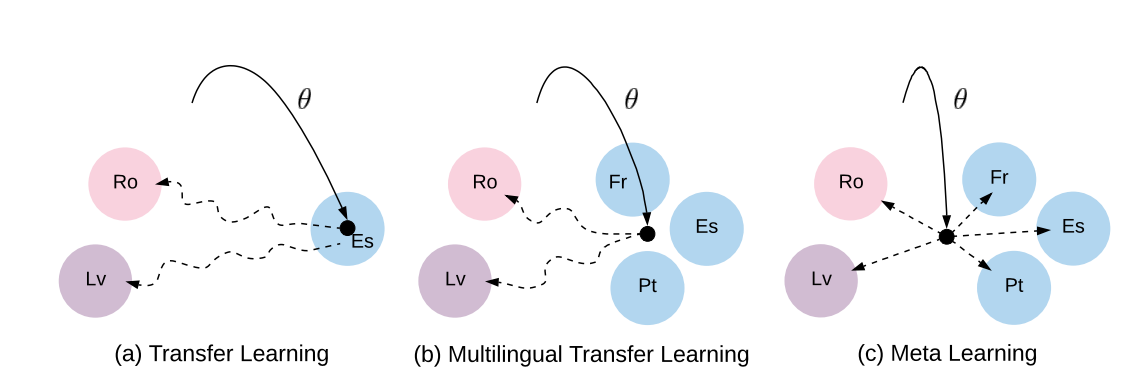
\includegraphics[width=0.9\textwidth]{fig/Meta-motivation.png}

  Our setting
  \begin{itemize}
    \item Language Adaptative Training
    \item End-to-end ASR: more realistic in low-resource regime
    \item Pluggable: no need to have target corpus during pretraining
  \end{itemize}
\end{frame}

\begin{frame}[t]{Implementation}
  \begin{itemize}
    \item Corpus: IARPA-BABEL (17 languages)
    \item Model structure: LAS
    \item Meta-learner: \textbf{Reptile}, FOMAML, Leap
  \end{itemize}
  \center 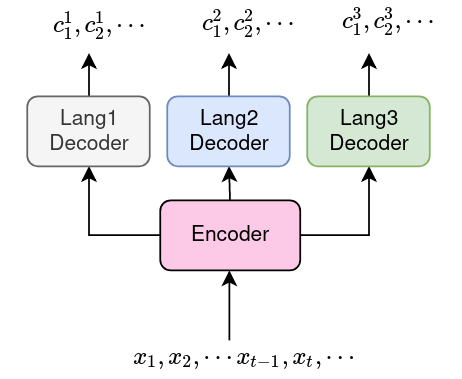
\includegraphics[width=0.5\textwidth]{fig/MultiTaskASR.png}
\end{frame}

\begin{frame}{Proposed method}
  Meta-learn
  \begin{itemize}
    \item Whole encoder
    \item Last layer of encoder (pretrain using multitask learning, then freeze till penultimate layers of encoder)
  \end{itemize}
  \pause
  \center 都失敗惹 QQ
\end{frame}

\section{Experiments on multitask learning}


\subsection{Pretraining language selection}
\begin{frame}{Hypothesis}
  Is it beneficial to choose \textbf{similar} languages during pretraining?
\end{frame}

\begin{frame}[t]{Lang2vec}
  \center 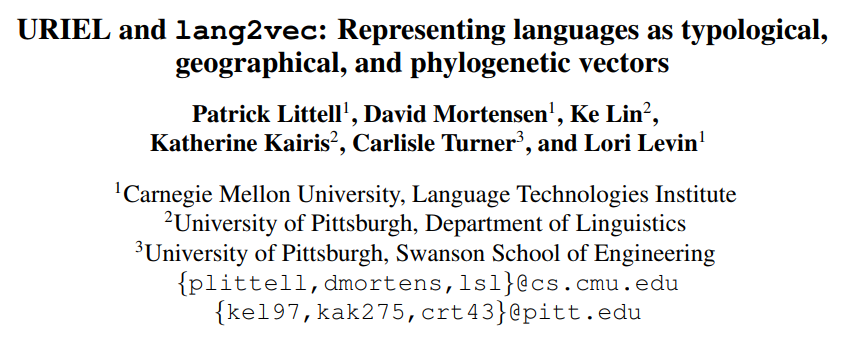
\includegraphics[width=\textwidth]{fig/lang2vec.png}
  \center 2017
\end{frame}

\begin{frame}{Mono Transfer Learning (CER on LLP)}
  Pretraining language selection
 \begin{table}[]
\begin{tabular}{lllllll}
\cline{2-6}
\multicolumn{1}{l|}{}            & \multicolumn{1}{l|}{Mono}  & \multicolumn{1}{l|}{PHN-near}             & \multicolumn{1}{l|}{PHN-far} & \multicolumn{1}{l|}{GEO-near}            & \multicolumn{1}{l|}{GEO-far}           &  \\ \cline{1-6}
\multicolumn{1}{|l|}{Bengali}    & \multicolumn{1}{l|}{66.1}  & \multicolumn{1}{l|}{66.5}                 & \multicolumn{1}{l|}{62.6}    & \multicolumn{1}{l|}{\textbf{59.8 (9\%)}} & \multicolumn{1}{l|}{62}                &  \\ \cline{1-6}
\multicolumn{1}{|l|}{Turkish}    & \multicolumn{1}{l|}{68.6}  & \multicolumn{1}{l|}{66.9}                 & \multicolumn{1}{l|}{64.6}    & \multicolumn{1}{l|}{\textbf{64.6 (6\%)}} & \multicolumn{1}{l|}{64.8}              &  \\ \cline{1-6}
\multicolumn{1}{|l|}{Tagalog}    & \multicolumn{1}{l|}{53.6}  & \multicolumn{1}{l|}{52.3}                 & \multicolumn{1}{l|}{49.3}    & \multicolumn{1}{l|}{49.1}                & \multicolumn{1}{l|}{\textbf{49 (9\%)}} &  \\ \cline{1-6}
\multicolumn{1}{|l|}{Vietnamese} & \multicolumn{1}{l|}{74.3}  & \multicolumn{1}{l|}{\textbf{51.9 (30\%)}} & \multicolumn{1}{l|}{54.8}    & \multicolumn{1}{l|}{54.7}                & \multicolumn{1}{l|}{54.4}              &  \\ \cline{1-6}
\multicolumn{1}{|l|}{Telugu}     & \multicolumn{1}{l|}{102.9} & \multicolumn{1}{l|}{\textbf{80.6 (21\%)}} & \multicolumn{1}{l|}{85}      & \multicolumn{1}{l|}{84.8}                & \multicolumn{1}{l|}{86.6}              &  \\ \cline{1-6}
\multicolumn{1}{|l|}{Lithuanian} & \multicolumn{1}{l|}{63.5}  & \multicolumn{1}{l|}{\textbf{59.3 (7\%)}}  & \multicolumn{1}{l|}{60}      & \multicolumn{1}{l|}{59.3}                & \multicolumn{1}{l|}{62.1}              &  \\ \cline{1-6}
                                 &                            &                                           &                              &                                          &                                        & 
\end{tabular}
%\caption{CER on LLP of IARPA-BABEL}
\label{tab:cer-trans}
\end{table}
\begin{itemize}
  \item Bengali, Turkish, Tagalog's \texttt{PHN-near}: Telugu
\end{itemize}
\end{frame}

\begin{frame}[t]{Multi Transfer Learning (CER on LLP)}
  Effect of pretraining step (Vietnamese for example)

    \begin{figure}[H]
    \centering
    \hspace{-5.2cm}
    \begin{tikzpicture}[trim axis left, trim axis right]

    \begin{axis}[
      width=0.6\linewidth,
      legend entries={Meta ASR (on \SI{10}{\percent} data), MultiTask ASR (on \SI{10}{\percent} data), no-pretrain (on \SI{10}{\percent} data),no-pretrain (on \SI{20}{\percent} data), no-pretrain (on \SI{50}{\percent} data)} ,
          xlabel = {Number of pretraining steps},
          xmin=0,
          xmax=210,
          grid=both,
          %legend style={at={(0.65,0.62)},anchor=south west},
          legend pos=outer north east,
          ylabel={Phoneme Classification Accuracy}]
    \addplot+[smooth]table{phn_near3};
    \addplot+[smooth]table{phn_far3};
     \addplot[style=ultra thick,dashed,] coordinates {(0,0.557) (200,0.557)};
     \addplot[style=ultra thick,dashed, gray] coordinates {(0,0.589) (200,0.589)};
     \addplot[style=ultra thick,dashed, brown] coordinates {(0,0.628) (200,0.628)};
    \end{axis}
    \end{tikzpicture}
    %\caption{Pretrain on EN, FI, FR, NL, RM, RU, and evaluate on }
    %\caption{TUNDRA phoneme classification experiment}
    \label{fig:tundra-exp}
  \end{figure}
    %\begin{figure}[H]
    %\centering
    %\hspace{-5.2cm}
    %\begin{tikzpicture}[trim axis left, trim axis right]

    %\begin{axis}[
      %width=0.6\linewidth,
      %legend entries={PHN-near3, PHN-far3} ,
          %xlabel = {Number of pretraining steps},
          %xmin=0,
          %xmax=210,
          %grid=both,
          %%legend style={at={(0.65,0.62)},anchor=south west},
          %legend pos=outer north east,
          %ylabel={CER}]
    %\addplot+[smooth]table{phn_near3};
    %\addplot+[smooth]table{phn_far3};
    %\end{axis}
    %\end{tikzpicture}
  %\end{figure}

\end{frame}



%\begin{frame}
  %\center It's important for multitask learning!
%\end{frame}



%\section{Meta-Learning With Latent Embedding Optimization}
%\begin{frame}
  %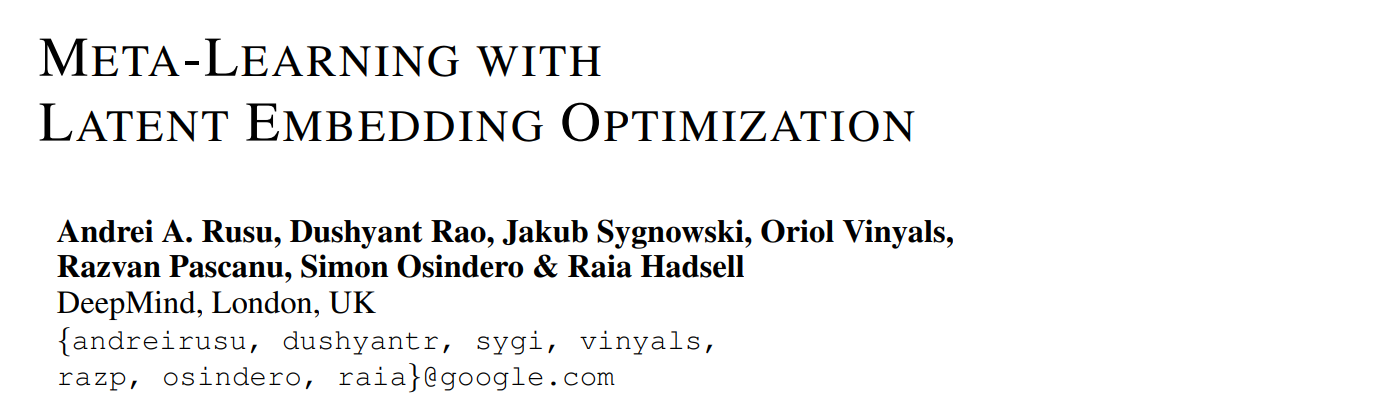
\includegraphics[width=\textwidth]{fig/LEO.png}
  %\center ICLR 2019
%\end{frame}



%\section{MISC}
\begin{frame}
	\begin{center}
    %\weib{\LARGE{謝謝聆聽!}}
    \LARGE{Questions?}
	\end{center}
\end{frame}

\end{document} 
